\documentclass[8pt]{beamer}
\usepackage{graphics}
\usepackage{amsmath,accents}
\usepackage{tikz}

\usetikzlibrary{angles, quotes, calc, decorations.markings, intersections}
\newcommand{\midlabelline}[3]{
	\node (midlabel) at ($ (#1)!.5!(#2) $) {#3};
	\draw[<-] (#1) --  (midlabel);
	\draw[->] (midlabel) -- (#2);
}
\usepackage{import}
\usetheme{Frankfurt}
\title{Finite Difference Method For Poisson Equation}
\date{\today}
\author{Akarsh Shukla , Brahmanand Mishra and Shashvat Jain}

\begin{document}
\maketitle

\section{Content}
\begin{frame}{Contents}

\begin{itemize}
\item Introduction 
\item Theory
\item Methodology
\item Analysis of Numerical Results
\item Summary 
\end{itemize}

\end{frame}

\section{Introduction}
\begin{frame}{Introduction}
	\begin{itemize}
		\item  Poisson Equation is an elliptic partial differential Equation.having general form as -: \\
	 \[  
		\frac{\partial^2 u}{\partial x^2} + \frac{\partial^2 u}{\partial y^2} =  f({r})
		\] \\
		\item Differential Equation can be converted into a system of linear equation by approxiamting them as derivatives by method of finite differences.
		\item There are many iterative schemes which can be employed to solve this system of linear equation such as Gauss Seidel, SOR and Jacobi Method.
		
		
	\end{itemize}
  
   
\end{frame}

\section{Theory}
	\subsection{Problem}
	\begin{frame}{Theory}
		\section{Problem}
		The below figure shows an interleaved capacitor -:
			\begin{figure}[h]
			\centering
			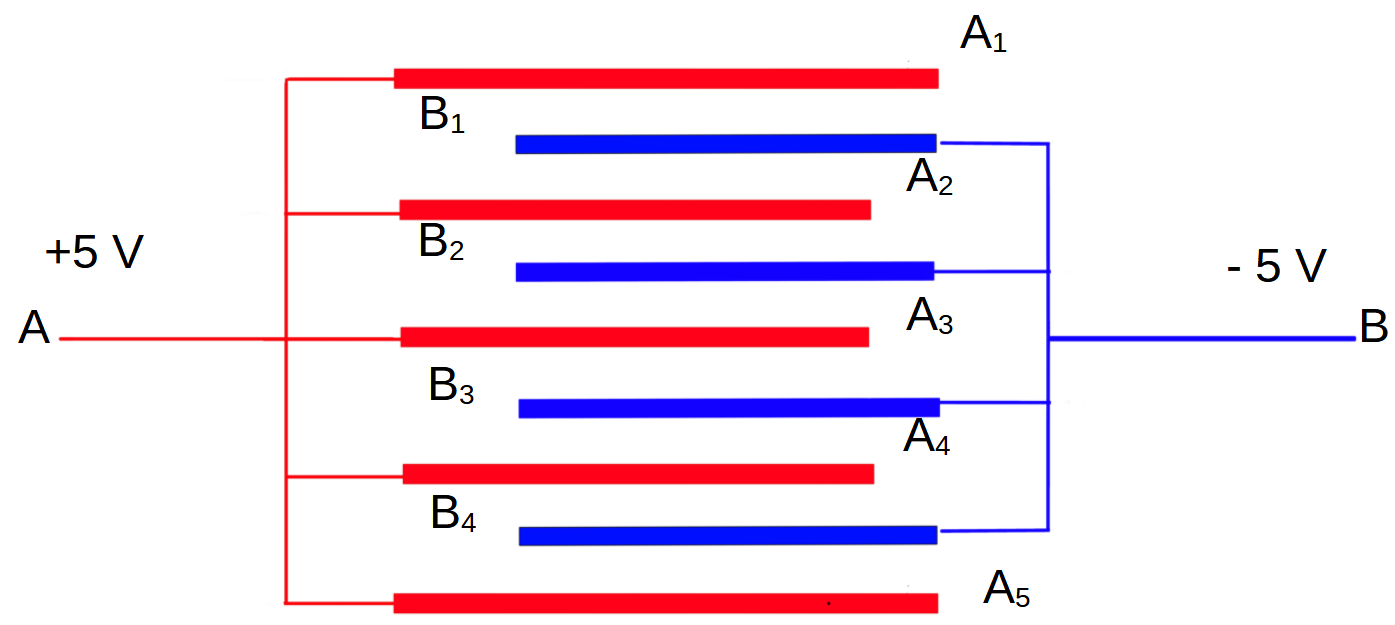
\includegraphics[width=2cm, height=1.9cm]{insert.png}
			\caption{\small Diagram dipciting the arrangement of plates in a interleaved fashion.}
			\label{fig 1: the capacitor}

			\end{figure}
			After non -dimensionalising we had following poisson equation-:
			$$ \frac{\partial^2U'(x',y') }{\partial x^{'2}} + \frac{\partial^2U'(x',y') }{\partial y^{'2}}= -\frac{\rho'(x',y') s^2}{\epsilon_0 \nu} $$
			
		\end{frame}
	\begin{frame}{Problem}
		\begin{equation}
			\rho'(x',y') =  \begin{cases}
				-2\epsilon_0 \times 10^5  & :\text{if} \; (x',y') \in B_i \; \text{where} \; i = 1,2,3,4 \\
				2\epsilon_0 \times 10^5 & :\text{if} \; (x',y') \in A_i \; \text{where} \; i = 2,3,4 \\
				0  & : \; \text{elsewhere}
			\end{cases}
		\end{equation}
		With boundary conditions as -:
		\begin{align}
			& U(0,y) = +5/\nu \quad \ U(4,y) = +5/\nu \\ 
			& U_y(x,0) = 0 \qquad \ U_y(x,4.4) = 0 
		\end{align}
		
		\end{frame}	
	\section{Methodology}
	\begin{frame}{Methodology}
		\subsection{Finite Differences}
		\begin{itemize}
			\item Finite Difference converts PDE into difference equation.
			\item Domain is converted into a mesh of equidistant grid points.
			\item Taylor series is used to approximate the value at  these grid points.
			 \item After using Finite Difference operators we get the following stencil for poisson equation
		\end{itemize}
		\begin{align}
			U_{i,j} = \frac{1}{4} \left[ U_{i+1,j}+ U_{i-1,j} + U_{i,j+1}+ U_{i,j+1} + h^2\frac{\rho'_{i,j} s^2}{\epsilon_0 \nu} \right]
		\end{align}
		This stencil can be represented with the help of following diagram -: \\
		\begin{figure}
			\centering
			
			\scalebox{0.4}{[
				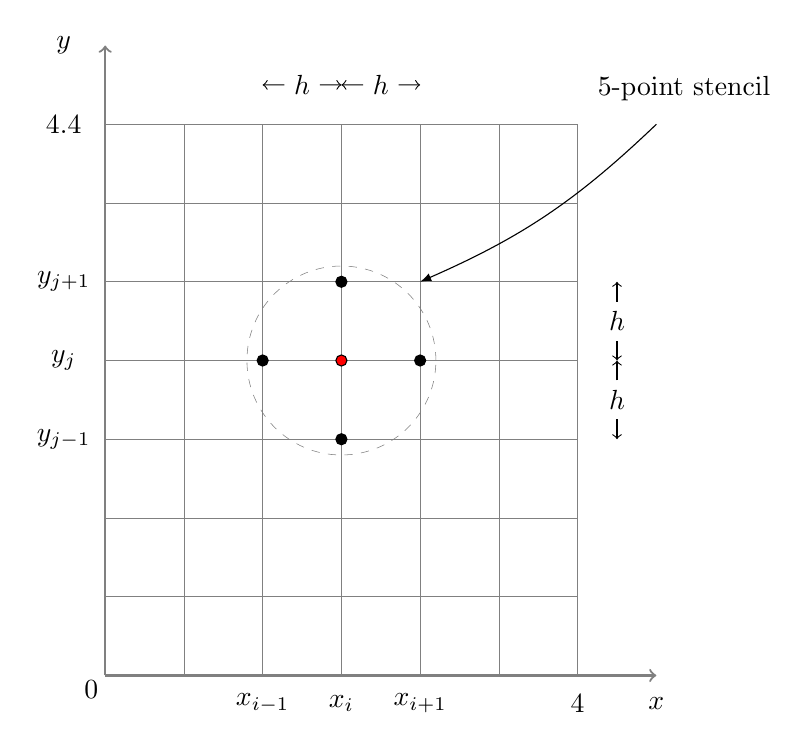
\begin{tikzpicture}
				\coordinate (Y) at (-15pt,8);
				\coordinate (X) at (7,-10pt);
				\draw[step = 1cm,gray, very thin] (0,0) grid (6,7);
				\draw[thick,color=gray,->] (0,0) -- (7,0);
				\draw[thick,color=gray,->] (0,0) -- (0,8);
				\draw (X) node {$x$};
				\draw (Y) node {$y$};
				\draw (X) node[shift={(-4,0)}] {$x_i$};
				\draw (Y) node[shift={(0,-4)}] {$y_j$};
				\draw (X) node[shift={(-5,0)}] {$x_{i-1}$};
				\draw (Y) node[shift={(0,-5)}] {$y_{j-1}$};
				\draw (X) node[shift={(-3,0)}] {$x_{i+1}$};
				\draw (Y) node[shift={(0,-3)}] {$y_{j+1}$};
				\draw (Y) node[shift={(0,-1)}] {$4.4$};
				\draw (X) node[shift={(-1,0)}] {$4$};
				\midlabelline{[shift={(-0.5,3cm + 10pt)}]X}{[shift={(-0.5,4cm +10pt)}]X}{$h$};
				\midlabelline{[shift={(-0.5,4cm +10pt)}]X}{[shift={(-0.5,5cm +10pt)}]X}{$h$};
				\coordinate (Xa) at ([shift={(2cm +15pt,-0.5)}]Y); 
				\coordinate (Xb) at ([shift={(3cm +15pt,-0.5)}]Y); 
				\coordinate (Xc) at ([shift={(4cm +15pt,-0.5)}]Y); 
				\midlabelline{Xa}{Xb}{$h$};
				\midlabelline{Xb}{Xc}{$h$};
				\draw (0,0) node[shift={(-5pt,-5pt)}] {$0$};
				\draw[fill=red] (3,4) circle (2pt) ;
				\draw[fill=black] (4,4) circle (2pt) ;
				\draw[fill=black] (2,4) circle (2pt) ;
				\draw[fill=black] (3,3) circle (2pt) ;
				\draw[fill=black] (3,5) circle (2pt) ;
				\draw[dashed,very thin,color=gray] (3,4) circle (1.2cm) ;
				\draw [latex-] (4cm,5cm) to [bend right=10] (7,7) node[anchor=south,shift={(10pt,5pt)}] {$5$-point stencil};
			\end{tikzpicture}]}
		\end{figure}
		\end{frame}	
		\subsection{Iterative Method }
		\begin{frame}{Iterative Method}
			\begin{itemize}
				\item Iterative methods are techniques that exploit the properites of system to solve it implicitly to make computation faster.
				\item We have used following iteratiion schemes-:\\
			
					 \begin{block}{Jacobi Method}
						This method starts with a guess value and with each iteration, it replace guess values with new obtained values from iteration.$$ x^{(n+1)}_{i,j} = S(X^{(n)},P,h,i,j) $$
						\end{block}
					 \begin{block}{Gauss Seidel Method}
						This method uses the obtained value in the same iteration for other unknowns.$$x^{(n+1)}_{i,j} = S(X^{(n+1)},P,h,i,j)$$
						\end{block}
					
					\begin{block}{SOR}
							This method involves a relaxation factor (greater than 1) which is multiplied to values obtained from Gauss Seidel before replacing old values.$$x^{(n+1)}_{i,j} = x^{(n)}_{i,j}+ \omega(S(X^{(n+1)},P,h,i,j)- x^{(n+1)}_{i,j})$$
							
						\end{block}
				
					
					\end{itemize}
				\end{frame}
			\section{result}
				\subsection{Expectation}
				\begin{frame}{Expectation}
					We expect the following graph-:\\
					\begin{itemize}
						\item $ \alpha_1 $ should decrease from positive to negative potential
						\item $ \alpha_2 $ should have negatively charged potential
						\item $ \alpha_3 $ should increase from negative to positive potential
						\item $ \alpha_4 $ should have positively charged  potential
					\end{itemize}
					
				\end{frame}
				\subsection{Numerical Result}
				\begin{frame}{Numerical Result}
					We obtained following graphs as solution -: \\
					
				\end{frame}
				\section{Conclusion}
					\begin{frame}
					
					\end{frame}
\end{document}

